\documentclass[11pt,letterpaper]{article}
\usepackage[margin=1in,headheight=14pt]{geometry}
\usepackage[T1]{fontenc}
\usepackage{lmodern}
\usepackage{amsmath,amssymb,amsthm,mathtools}
\usepackage{microtype,booktabs,tikz,xcolor,fancyhdr}
\definecolor{ink}{HTML}{19354A}
\definecolor{rust}{HTML}{B65E3B}
\definecolor{teal}{HTML}{28786E}
\definecolor{violet}{HTML}{87619E}
\definecolor{gold}{HTML}{B58524}
\definecolor{slate}{HTML}{647F9B}
\usepackage[colorlinks=true,linkcolor=ink,urlcolor=ink]{hyperref}
\hypersetup{
  pdftitle={Rainbow perfect matchings on even cycles and two disjoint squares},
  pdfauthor={Akhil Ravuri},
  pdfsubject={Elementary combinatorics exposition}
}
\newtheorem{theorem}{Theorem}
\newcommand{\Next}{N_{\mathrm{ext}}}
\pagestyle{fancy}
\fancyhf{}
\fancyhead[L]{\small\textsc{Rainbow perfect matchings}}
\fancyhead[R]{\small Akhil Ravuri}
\fancyfoot[C]{\thepage}
\renewcommand{\headrulewidth}{0.3pt}
\setlength{\parindent}{1.2em}
\setlength{\parskip}{0.25em}
\setlength{\emergencystretch}{1em}
\allowdisplaybreaks[1]
\title{\vspace{-1.5em}\LARGE\bfseries Rainbow perfect matchings\par
  \Large on even cycles and two disjoint squares}
\author{Akhil Ravuri}
\date{}

\begin{document}
\maketitle
\vspace{-1.5em}
\begin{abstract}
We determine the maximum number of colors in an edge coloring of an even
cycle that avoids a rainbow perfect matching, and count all extremal
partitions of its fixed edge set. For two disjoint squares, we prove that
the maximum is six and that exactly two extremal partitions occur.
The arguments are elementary and self-contained; no novelty is claimed.
\end{abstract}

\section{Definitions and the even-cycle formula}
All graphs are finite and simple, and edge colorings need not be proper.
A perfect matching is \emph{rainbow} if its edges have pairwise distinct
colors. For a graph $G$ admitting an avoiding coloring, let $A(G)$ be the
maximum number of colors in a coloring with no rainbow perfect matching.
Let $\Next(G)$ count the color-class partitions attaining this maximum.
Throughout, the edge set is fixed: color names are ignored, but partitions
related by vertex symmetries are not identified.

\begin{theorem}\label{thm:cycles}
For every integer $n\ge 2$,
\[
  A(C_{2n})=2n-2,
  \qquad
  \Next(C_{2n})=\binom{n}{2}^{\!2}.
\]
\end{theorem}

\begin{proof}
An even cycle has exactly two perfect matchings, $M_1$ and $M_2$.
Once the matching edge at one vertex is chosen, the remaining choices
around the cycle are forced. These are the two alternating sets of edges,
and they partition $E(C_{2n})$.

Let $S_i$ be the set of colors on $M_i$. In an avoiding coloring, neither
matching is rainbow, so $|S_i|\le n-1$. Thus
\[
  |S_1\cup S_2|\le |S_1|+|S_2|\le 2n-2.
\]
Conversely, choose one pair of edges in each matching and give that pair
a common color. Give every remaining edge its own color, using disjoint
palettes between the matchings. This uses $2n-2$ colors and avoids a rainbow
perfect matching, proving the formula for $A$.

Equality forces $|S_1|=|S_2|=n-1$ and $S_1\cap S_2=\varnothing$.
A partition of $n$ edges into $n-1$ nonempty classes has exactly one
class of size two and otherwise singletons. Hence each matching has one
repeated pair. Choosing the two pairs independently gives
$\binom{n}{2}^2$ distinct edge partitions, and every extremal partition
arises uniquely this way.
\end{proof}

\newpage
\section{The maximum for two disjoint squares}
Let $G=H_1\sqcup H_2$, where $H_1$ and $H_2$ are fixed copies of $C_4$.
A perfect matching of $G$ is the union of a perfect matching in each
component. There are therefore exactly four global perfect matchings.

\begin{theorem}\label{thm:squares-bound}
For $G=C_4\sqcup C_4$, we have $A(G)=6$.
\end{theorem}

\begin{proof}
Color the cyclically ordered edges of $H_1$ with $A,B,A,B$ and give the four
edges of $H_2$ four distinct new colors. Every global perfect matching
contains one of the two monochromatic local matchings of $H_1$.
Thus six colors are attainable without a rainbow perfect matching.

\begin{center}
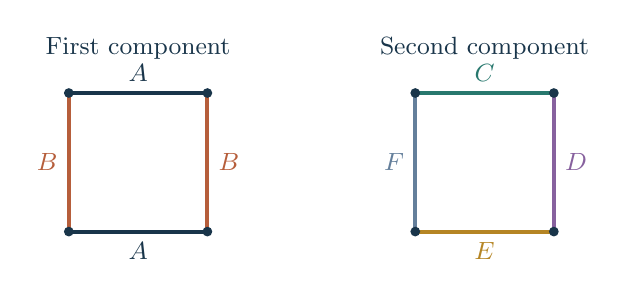
\begin{tikzpicture}[scale=0.88,every node/.style={font=\small}]
  \node[text=ink] at (1,2.65) {First component};
  \node[text=ink] at (6,2.65) {Second component};
  \draw[ink,line width=1.5pt] (0,2)--node[above] {$A$} (2,2);
  \draw[rust,line width=1.5pt] (2,2)--node[right] {$B$} (2,0);
  \draw[ink,line width=1.5pt] (2,0)--node[below] {$A$} (0,0);
  \draw[rust,line width=1.5pt] (0,0)--node[left] {$B$} (0,2);
  \draw[teal,line width=1.5pt] (5,2)--node[above] {$C$} (7,2);
  \draw[violet,line width=1.5pt] (7,2)--node[right] {$D$} (7,0);
  \draw[gold,line width=1.5pt] (7,0)--node[below] {$E$} (5,0);
  \draw[slate,line width=1.5pt] (5,0)--node[left] {$F$} (5,2);
  \foreach \x in {0,2,5,7} \foreach \y in {0,2}
    \fill[ink] (\x,\y) circle (2pt);
\end{tikzpicture}

\small An avoiding six-coloring: the first square forces a repeated color.
\end{center}

For the upper bound, consider a coloring using at least seven colors on
the eight edges. With eight colors, every perfect matching is rainbow.
With seven, precisely two edges $e,f$ share a color and all other classes
are singletons. In the component containing $e$, choose the alternating
matching omitting $e$, and combine it with either matching of the other
component. The resulting perfect matching omits $e$, so it cannot contain
the only repeated pair. It is rainbow, proving the upper bound.
\end{proof}

\section{Characterizing the extremal partitions}
\begin{theorem}\label{thm:squares-count}
With edge positions fixed and color names ignored,
$\Next(C_4\sqcup C_4)=2$.
\end{theorem}

\begin{proof}
A six-color partition of eight edges has class sizes $s_1,\dots,s_6$ with
$\sum_{i=1}^{6}(s_i-1)=2$. Thus the only possible size patterns are
\[
  (3,1,1,1,1,1)
  \quad\text{or}\quad
  (2,2,1,1,1,1).
\]
\emph{Excluding the triple.}
Every edge belongs to exactly two of the four global perfect matchings.
Three equal-colored edges therefore have six total appearances across
those matchings. To obstruct every matching, each would have to contain
at least two of the three edges, requiring at least eight appearances.
This contradiction rules out a triple.

\newpage
\noindent\emph{Two repeated pairs.}
Let $P$ and $Q$ be the two doubleton color classes. A perfect matching is
non-rainbow exactly when it contains $P$ or $Q$ in full. The number of
global perfect matchings containing a given pair is as follows.

\begin{center}
\renewcommand{\arraystretch}{1.15}
\begin{tabular}{@{}lc@{}}
\toprule
Pair position & Number of matchings \\
\midrule
Adjacent edges in one component & $0$ \\
Opposite edges in one component & $2$ \\
One edge in each component & $1$ \\
\bottomrule
\end{tabular}
\end{center}

Adjacent edges cannot occur together. Opposite edges specify one local
matching, leaving two choices in the other component. One edge in each
component specifies both local choices, giving exactly one global matching.

Together, the two pairs must obstruct all four matchings. Each pair
obstructs at most two, so both must obstruct exactly two, with their
obstructed sets disjoint. Hence each pair consists of opposite edges in
one component. If the pairs belonged to different components, choosing
the other local matching in each component would give a rainbow global
matching. Both pairs must therefore lie in the same component.

Since the color classes are disjoint, the pairs must be precisely that
component's two alternating perfect matchings. There are two choices for
this component; the other component has four singleton classes. Each
choice avoids a rainbow perfect matching, and the choices define distinct
fixed-edge partitions. Renaming or interchanging colors adds no further
partitions, so the count is two.
\end{proof}

\section{Small cases and computational checks}
The preceding proofs give the following values.
\begin{center}
\renewcommand{\arraystretch}{1.15}
\begin{tabular}{@{}lcc@{}}
\toprule
Host $G$ & $A(G)$ & $\Next(G)$ \\
\midrule
$C_4$ & $2$ & $1$ \\
$C_6$ & $4$ & $9$ \\
$C_8$ & $6$ & $36$ \\
$C_{10}$ & $8$ & $100$ \\
$C_4\sqcup C_4$ & $6$ & $2$ \\
\bottomrule
\end{tabular}
\end{center}
The repository's documented sparse search also checks $C_4$, $C_6$, $C_8$,
and the disjoint squares, agreeing with these formulas. The $C_{10}$ row
is a consequence of the proof; no additional computation is claimed here.
Computation is not a premise of any theorem in this note.

For the edge order, raw data, reproduction commands, and execution limits,
see \href{https://github.com/Akhil-rav/discrete-math-lab/pull/1}{Discrete Math
Lab, PR~\#1}, especially the following files:
\begin{quote}\small
\nolinkurl{results/data/sparse_rainbow.json}\\
\nolinkurl{results/sparse_verification.md}
\end{quote}
These counts concern color partitions on fixed edges, not graph
isomorphism classes.
\end{document}
